\section{What are the mathematical foundations of a ConvNet?}
\label{sec:math}

There are many fields of mathematics that contribute to the functionality of neural networks. They depend heavily on linear algebra, probability theory, and optimization. ConvNets use multiple kinds of mathematics as well. However, in this section we will focus on the operation that gives convolutional neural networks their name.

\subsection{Convolution integral}

One of the most important operations in a ConvNet is the convolution operation. This mathematical operation is a way to blend two functions together \cite{wolf} and can be used continuously or discretely. It is often denoted by the symbol $*$. A possible definition for the continous case is:

\begin{equation}\label{eq:convo}
    [f * g] (t) = \int_{-\infty}^{\infty} f(\tau)g(t-\tau) d\tau.
\end{equation}

The first mathematician to have written down a convolution was presumably D'Alembert in 1754 \cite{tor}, albeit in a different form. In 1807, Fourier used a convolution in a form similar to equation \eqref{eq:convo}. To get a sense of the idea behind a convolution let us look at an enlightening example, paraphrased from \cite[Ch. 9]{dl-book}:\\

\textit{Suppose we are tracking the location of a spaceship with a continuous laser sensor, which outputs the position $x(t)$ at time $t$. If the sensor is a bit noisy, we want to average the measurements. To give recent measurements more importance, we use a weight function $w(a)$ based on the age $a$ of the measurement. The smoothed estimate $s(t)$ of the position of the spaceship becomes:
}
\begin{equation}
    s(t) = [x*w](t) = \int_{-\infty}^{\infty} x(\tau)w(t-\tau)d\tau.
\end{equation}

The weight function $w(a)$ would need to be a probability density function (pdf) to make $s(t)$ a proper weighted average. For instance, the exponential distribution has a suiting pdf, also because negative ages (i.e. looking into the future) would get a weight of zero.\\


\subsection{Discrete convolutions}

Convolutions do not have to be based on time, it could be any kind of variable. An option that is often used in the applications of ConvNets is \textit{location}, specifically the location of a pixel on an image. The convolution now has two dimensions since a pixel location is indicated by row $i$ and column $j$. The integral will be discretized, and the commutative property of convolution is used to arrive at:

\begin{equation}\label{eq:sums}
    S(i,j) = \sum_m \sum_n I(i-m,j-n)K(m,n).
\end{equation}

The function $I(i,j)$ stands for the input, analogous to the previous $x(t)$, and $K(i,j)$ is called the kernel, much alike the weights from before. In the simplified example of \autoref{fig:kern} the indices $m$ and $n$ from equation \eqref{eq:sums} both run over three different values. The kernel thus has a size of 3x3 in this case, with the values:

\begin{equation*}
    K = 
    \begin{bmatrix}
        1 & 0 & 1 \\
        0 & 1 & 0 \\
        1 & 0 & 1 \\
    \end{bmatrix}.
\end{equation*}

\begin{figure}
    \centering
    \animategraphics[width=0.8\textwidth,keepaspectratio,autoplay,loop]{0.8}{images/kernel/}{0}{9}
    \caption{Computations done by a discrete convolution. Source: \cite{stanf}. Open this pdf file in Adobe Acrobat Reader to see the animation.}
    \label{fig:kern}
\end{figure}

The kernel gets multiplied with a subset of the image in an element-wise fashion, much like the Hadamard product for matrices. Except in this case the outcomes are all summed together to form one pixel in the convolved feature map.\\

The discrete version of the convolution integral was probably introduced many years later than its continuous sibling. It is difficult to say exactly when, but one of the first appearances of a discrete convolution that we know of was penned by Cauchy in 1821 \cite{tor}. It has been employed in probability, statistics, and it's seen as the most important technique in digital signal processing \cite[Ch. 6]{dsp}.\\

Within ConvNets, the convolutions are used to extract certain features of an image. For example, the kernel from equation \eqref{eq:outline} can be used to get a more focussed outline of a picture \cite{visual}. In \autoref{fig:outline} you see the outcome of one convolution layer applied to the earlier picture of Dr. Fukushima. These edges within an image help to classify the content of the image in deeper layers of the ConvNet.

\begin{equation}\label{eq:outline}
    K =
    \begin{bmatrix}
     -1 & -1 & -1 \\
     -1 & 8 & -1 \\
     -1 & -1 & -1 \\
    \end{bmatrix}.
\end{equation}

\begin{figure}
    \centering
    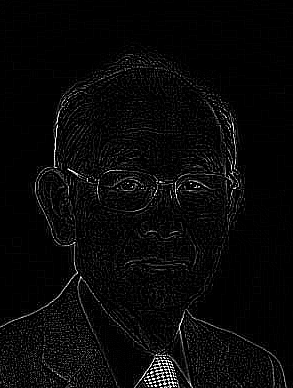
\includegraphics[width=0.45\textwidth]{images/Fukushima-outline.png}
    \caption{The outlines of Fukushima's portret. Made with \cite{visual}}
    \label{fig:outline}
\end{figure}



%more about discrete conv on page 19:

%https://www.slideshare.net/Alexdfar/origin-adn-history-of-convolution









